\newpage
\section{Design patterns}

\subsection{Strutturali}
\subsubsection{Facade}
\textbf{Scopo}	Permette, attraverso un'interfaccia più semplice, l'accesso a sottosistemi che espongono interfacce complesse e molto diverse tra loro, nonché a blocchi di codice complessi. Questo rende una libreria più facile da capire, usare e testare, inoltre permette di diminuire le dipendenze tra sottosistemi senza nascondere le funzionalità di basso livello.
\\\\
\textbf{Motivazione}	L'utilizzo del pattern \textit{Facade\ped{G}} permette di nascondere la complessità del'operazione. Quando un sistema complesso viene strutturato in sottosistemi, le dipendenze rischiano di aumentare in modo consistente. Applicare il pattern \textit{Facede\ped{G}} aiuta a diminuire queste dipendenze. Il sottosistema possederà un'interfaccia semplificata che il \textit{client\ped{G}} utilizza anziché dover gestire numerosi oggetti. Utilizzare il pattern \textit{Facade\ped{G}} promuove un accoppiamento debole tra sottosistema ed i \textit{client\ped{G}}, che comporta una maggiore flessibilità nello sviluppo: è possibile modificare il sottosistema senza che i \textit{client\ped{G}} debbano adeguarsi a loro volta. \\
Ciononostante i \textit{client\ped{G}} possono comunque accedere alle funzionalità di basso livello ed utilizzare le classi del sottosistema.
\\\\
\textbf{Applicabilità}	Il pattern \textit{Facade\ped{G}} si usa nei seguenti casi:
	\begin{itemize}
		\item Si vuole fornire una singola interfaccia semplice per un sottosistema complesso;
		\item Si vuole promuovere il disaccoppiamento tra sottosistemi e \textit{client\ped{G}}, semplificando le dipendenze;
		\item Si vuole stratificare un sistema: è possibile definire una classe \textit{Facade\ped{G}} come punto d'ingresso per ogni livello di sottosistema. In questo modo, se vi sono dipendenze fra sottosistemi, essi possono comunicare fra loro attraverso la propria \textit{Facade\ped{G}}.
	\end{itemize}
	
\textbf{Utilizzo}

\subsection{Creazionali}
\subsubsection{Dependecy Injection}
\textbf{Scopo}	Semplificare lo sviluppo e rendere più testabile un software di grandi dimensioni. Il pattern \textit{Dependency Injection\ped{G}} separa il codice della componente dal codice che si occupa di risolvere le dipendenze con altre componenti.
\\\\
\textbf{Motivazione}	Lasciare al componente il compito di risolvere le proprie dipendenze, creando gli oggetti necessari al suo funzionamento, aumenta l'accoppiamento tra le componenti e rende più difficoltoso progettare i test di unità.
\\ Con questo pattern invece è possibile esprimere le dipendenze in modo dichiarativo e utilizzare un oggetto \textit{contenitore} per risolverle dinamicamente a \textit{runtime\ped{G}}. In questo modo è possibile scegliere anche quale componente iniettare in base allo stato del programma.
\\\\
\textbf{Applicabilità}	Questo pattern viene utilizzato dalla maggior parte dei \textit{framework\ped{G}} moderni. In particolare, \textit{AngularJS\ped{G}} offre il servizio
\\\\
\texttt{injector} che permette di invocare delle funzioni iniettando al loro interno degli oggetti.
\\\\
\textbf{Utilizzo}
\\\\
\textbf{Struttura}	I componenti coinvolti nel \textit{Dependency Injection} sono:
	\begin{itemize}
		\item Un \textit{client\ped{G}} che viene creato e riceve le dipendenze;
		\item Un \textit{contenitore} che si occupa di creare il \textit{client\ped{G}} e di iniettarvi le dipendenze;
		\item Un \textit{servizio} che deve essere iniettato al \textit{client\ped{G}}.
	\end{itemize}
Nello specifico di \textit{AngularJS\ped{G}} \texttt{Injector} funziona da \textit{contenitore} che si occupa di risolvere le dipendenze. I \textit{client\ped{G}} sono rappresentati dalle funzioni che costruiscono i componenti dell'applicazione, tipicamente \textit{controller\ped{G}} o \textit{service\ped{G}}. Il \textit{servizio} è un oggetto \textit{service} che può essere definito dall'utente oppure uno di quelli resi disponibili da \textit{AngularJS\ped{G}}.
\label{Struttura logica del pattern Dependency Injection}
\begin{figure}
	\centering
	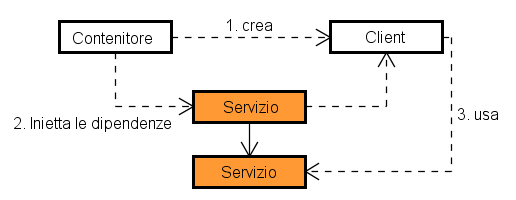
\includegraphics[scale=0.45]{UML/strutturaPattern/DependencyInjection.png}
	\caption{Struttura logica del pattern Dependency Injection}
\end{figure}
\\\\
\textbf{Collaborazioni}
\\\\
\textbf{Svantaggi}	Eventuali errori legati alla risoluzione delle dipendenze o alla loro implementazione vengono rilevati solamente a \textit{runtime\ped{G}}.


\subsection{Comportamentali}
\subsubsection{Chain-of-responsability}
\textbf{Scopo}	Il pattern \textit{Chain-of-responsability\ped{G}} ha lo scopo di evitare l'accoppiamento tra il mittente di una richiesta e il destinatario, in modo che più di un singolo oggetto possa eseguire la richiesta. Concatenare gli oggetti destinatari e passare la richiesta di oggetto in oggetto, finché uno di questi non riesce ad esaudirla.
\\\\
\textbf{Motivazione}	L'oggetto che ha iniziato la richiesta non è a conoscenza di chi la esaudirà, per questo si parla di destinatario implicito. Ogni oggetto della catena condivide un'interfaccia comune \textit{handler} per la gestione delle richieste e per accedere al successivo elemento della catena. Questo per consentire il passaggio lungo la catena e per assicurare che l'oggetto che eventualmente esaudirà la richiesta rimanga implicito. Il metodo che viene mantenuto in tutte le interfacce per creare la catena si chiama \textit{handle}. \textit{handle}, nella versione standard, esegue la chiamata al successore della catena. Alla fine della catena viene fatto l'ovverriding\ped{G} di questo metodo, implementando la richiesta iniziale oppure generando l'errore.
\\\\
\textbf{Applicabilità}	\textit{Chain-of-responability} si usa nei seguenti casi:
	\begin{itemize}
		\item Più di un oggetto può gestire la richiesta ed il ricevente che la gestirà non è conosciuto a priori;
		\item Si vuole passare una richiesta ad uno dei molti oggetti, senza esplicitare il ricevente;
		\item L'insieme di oggetti che gestirà una richiesta deve essere definito dinamicamente.
	\end{itemize}
\textbf{Utilizzo}	Express una \textit{Chain-of-responsability} per la gestione dei middleware e del routing. Nell'architettura viene utilizzato all'interno del package \textit{Back-End\ped{G}}::App. Ogni \textit{ConcreteHandler} eredita da \textit{MiddlewareHandler}, che corrisponde all'interfaccia astratta \textit{Handler} del design pattern. Con Express i middleware corrispondono ai \textit{ConcreteHandler}. L'implementaizone di questi risulta sotto alcuni aspetti differente da una normale implementazione del pattern:
	\begin{enumerate}
		\item I middleware di express possono essere delle classi che implementano il metodo \textit{handle} oppure delle funzioni secondo lo stile funzionale delle \textit{librerie\ped{G}} e dei moduli di Node.js. Nella nostra architettura abbiamo utilizzato principalmente la seconda verisone;
		\item Nel \textit{design pattern\ped{G}} è previsto che l'oggetto \textit{ConcreteHandler} abbia un riferimento (successor) al \textit{ConcreteHandler} successivo. Express, anzichè un riferimento, passa al metodo che esegue il middleware una \textit{callback\ped{G}}. Il middleware che esegue la \textit{callback\ped{G}} passa il controllo all'oggetto del \textit{server\ped{G}} di Express, il quale passerà a sua volta il controllo al successivo middleware.
	\end{enumerate}
Express divide i middleware in due tipologie:
	\begin{enumerate}
		\item \textit{Middleware standard} con 3 parametri formali;
		\item \textit{Middleware per la gesitone delgi errori} con 4 parametri formali, ovvero i 3 del middleware standard più un parametro per gli errori.
	\end{enumerate}
Ogni middleware può passare il controllo ai middleware standard successivo, oppure ad un middleware per la gestione degli errori, passandogli l'errore relativo. Ogni middleware di Express deve essere invocato con i parametri elencati \textbf{nel seguente ordine:}
	\begin{enumerate}
		\item L'eventuale errore da gestire, in caso si tratti di un middleware per la gestione degli errori;
		\item L'oggetto contenente la richiesta da risolvere;
		\item L'oggetto che conterrà la risposta;
		\item La \textit{callback\ped{G}} da utilizzare per passare il controllo al successivo middleware.
	\end{enumerate}

\textbf{Struttura}
\label{Struttura logica del pattern Chain-of-responsability}
\begin{figure}
	\centering
	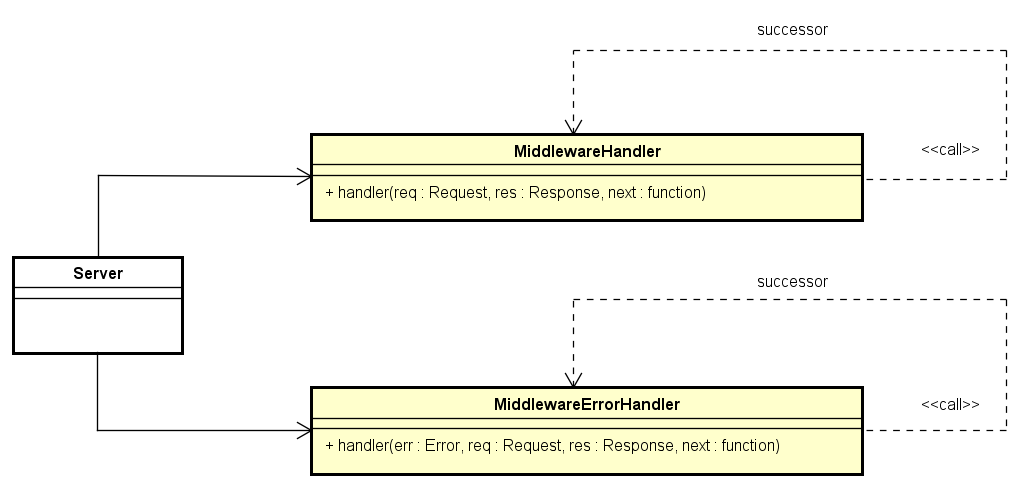
\includegraphics[scale=0.50]{UML/strutturaPattern/Chain-of-responsability.png}
	\caption{Struttura logica del pattern Chain-of-responsability}
\end{figure}

\textbf{Collaborazioni}		Quando un \textit{client\ped{G}} effettua una richiesta, questa viene propagata lungo la catena finché un \textit{ConcreteHandler} non si assume la responsabilità di gestirla.
\\\\
\textbf{Svantaggi}	È necessario porre attenzione a come si configura la catena. Infatti, in caso di configurazione inappropriata, sussiste il rischio che la richiesta passi per diversi putni della catena senza essere mai realizzata, oppure che la richiesta non venga realizzata perché non esiste un \textit{ConcreteHandler} che la possa risolvere.


\subsubsection{Iterator}
\textbf{Scopo}	Il design pattern \textit{iterator\ped{G}} risolve diversi problemi connessi all'accesso e alla navigazione attraverso gli elementi di una struttura dati contenitrice, senza esporre i dettagli dell'implementazione e della struttura interna del contenitore
\\\\
\textbf{Motivazione}	Un'alternativa semplice e preferibile all'uso di indici (come accade ad esempio per gli array) consiste nell'aggiungere operazioni all'interfaccia del contenitore. Questa soluzione ha il grosso vantaggio che, se l'interfaccia è ben definita, consente di annullare la dipendenza da dettagli interni del contenitore, ma ciò presenta alcuni inconvenienti:
	\begin{itemize}
		\item \textit{Sovraccarico del'interfaccia del contenitore:} le operazioni aggiunte sovraccaricano l'interfaccia preesistente della classe contenitore;
		\item \textit{Mancanza di punti di accesso multipli:} le operazioni sono centralizzate nella classe contenitore. Questo non consente di effettuare contemporaneamente più visite indipendenti dagli elementi dello stesso contenitore;
		\item \textit{Supporto carente per metodi di navigazione specializzati:} quando i contenitori possiedono una struttura complessa, non di rado vi sono diversi e ugualmente utili modi di attraversarne l'insieme degli elementi contenuti. Un'interfaccia centralizzata si adatta male a questa situazione, perché richiede l'aggiunta di più operazioni specializzate, esacerbando il problema del sovraccarico.
	\end{itemize}
\textbf{Applicabilità}	Il design pattern \textit{iterator\ped{G}}, quindi, supera le soluzioni che si possono ottenere con la pura programmazione ad oggetti mediante codice più complesso.
\\
\textbf{Struttura}	Il pattern \textit{iterator\ped{G}} definisce due gerarchie di classi: una per i contenitori e una per gli iteratori\ped{G}. Le classi contenitore possono essere specializzate per tipo di elemento contenuto o per tipo di struttura in cui gli elementi sono organizzati. Le classi di iteratori\ped{G} sono specializzati per tipo di contenitore (iteratore\ped{G} concreto) e per tipo di navigazione attraverso la sequenza di elementi (iteratori\ped{G} specializzati).
\\
\label{Struttura logica del pattern Iterator}
\begin{figure}
	\centering
	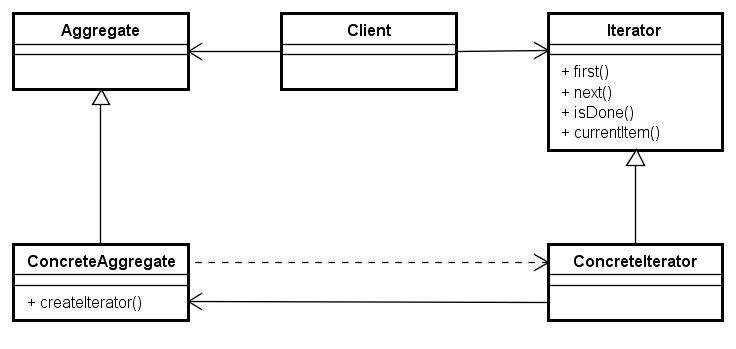
\includegraphics[scale=0.45]{UML/strutturaPattern/Iterator.png}
	\caption{Struttura logica del pattern Iterator}
\end{figure}
\\
\textbf{Collaborazioni}	Il design pattern \textit{iterator\ped{G}} richiede la collaborazioni di alcuni elementi:
	\begin{itemize}
		\item \textbf{Iterator:} definisce un'interfaccia per attraversare l'insieme degli elementi di un contenitore e accedere ai singoli elementi;
		\item \textbf{ConcreteIterator:} implementa l'interfaccia \textit{iterator\ped{G}} tenendo traccia della posizione corrente nel contenitore e calcolando qual'è l'elemento successivo nella sequenza di attraversamento;
		\item \textbf{Aggregate:} definisce un'interfaccia per creare un oggetto \textit{iterator\ped{G}}.
		\item \textbf{ConcreteAggregate:} implementa l'interfaccia di creazione dell'\textit{iterator} e ritorna un'istanza appropriata di \texttt{ConcreteIterator}.
	\end{itemize}
\textbf{Svantaggi}	L'utilizzo del design pattern \textit{iterator\ped{G}} rende più complesso il codice e di conseguenza meno leggibile.


\subsubsection{Observer}
\textbf{Scopo}	Definisce una dipendenza “1..n” fra oggetti, riflettendo la modifica di un oggetto sui dipendenti.
\\\\
\textbf{Motivazione}	In alcuni casi è necessario tenere sincronizzati vari oggetti e, nel caso un oggetto venga modificato, avere la possibilità di riflettere il cambiamento sugli oggetti dipendenti. \\ Il pattern \textit{Observer\ped{G}} permette di implementare ciò definendo due tipologie di oggetti: i \textit{subject}, che rappresentano gli oggetti osservati, e gli \textit{observer\ped{G}} che rappresentano gli oggetti che osservano lo stato del \texttt{subject}. Con questo pattern è possibile quindi realizzare un sistema \textit{publish-subscribe}, nel quale i vari \textit{subject} si registrano per essere notificati dalle modifiche subite dal \textit{subject}.
\\\\
\textbf{Applicabilità}	Il pattern \textit{observer\ped{G}} viene usato nei seguenti casi:
	\begin{itemize}
		\item Si vuole che il cambiamento dello stato di un oggetto provochi l'aggiornamento di altri oggetti;
		\item Si vuole notificare degli oggetti dell'avvenimento di un determinato evento senza sapere il loro tipo.
	\end{itemize}

\textbf{Utilizzo}

\subsection{Architetturali}
\subsubsection{MVC}
\textbf{Scopo}
\textbf{Motivazione}
\textbf{Applicabilità}
\textbf{Utilizzo}
\textbf{Struttura}
\textbf{Collaborazioni}
\textbf{Svantaggi}
